%Dạng 44
\setcounter{section}{43}
\setcounter{ex}{0}
\section{Diện tích hình phẳng}
\subsection{Kiến thức cần nhớ}
\begin{khung}
\subsubsection{Ứng dụng tích phân tính diện tích}
	\begin{enumerate}
		\item Một số hình thức đề cho và hướng xử lý trong trắc nghiệm
		\begin{itemize}
			\item Hình thức 1: Không cho hình vẽ, cho dạng $(H) : \left\{y=f(x), y=g(x), x=a, x=b\ (a<b)\right\}\xrightarrow{\text{ casio }}\displaystyle\int\limits_{a}^{b}\left|f(x)-g(x) \right|\mathrm{\,d}x =$ kết quả, so sánh với bốn đáp án.
			\item Hình thức 2: Không cho hình vẽ, cho dạng $(H):\left\{y=f(x), y=g(x)\right\}$. Giải  $f(x)=g(x)\Rightarrow x_1, \ldots, x_i$ với $x_1$ nhỏ nhất, $x_i$ lớn nhất  $\xrightarrow{\text{ casio }}\displaystyle\int\limits_{x_1}^{x_i}\left|f(x)-g(x) \right|\mathrm{\,d}x $
			\item Hình thức 3:  Cho hình vẽ, sẽ giải phương trình tìm tọa độ giao điểm  ( nếu chưa cho trên hình), chia từng diện tích nhỏ, xổ hình từ trên xuống, ghi công thức và bấm máy tính. 
			\item Hình thức 4: Cho ba hàm trở lên, chẳng hạng $y=f(x), y=g(x), y=h(x)$ ta nên vẽ hình.
		\end{itemize} 
	\end{enumerate}
\subsubsection{Ứng dụng tính thể tích khối tròn xoay}
\begin{enumerate}
	\item Thể tích vật thể(mặt cắt)\\
	Gọi $B$ là phần vật thể giới hạn bởi hai mặt phẳng vuông góc với trục $Ox$ tại các điểm $a$ và $b$, $S(x)$ là diện tích thiết diện của vật thể bị cắt bởi mặt phẳng vuông góc với trục $Ox$ tại điểm $x$, ($a\le x\le b$). Giả sử $S(x)$ là hàm số liên tục trên đoạn $[a;b]$. Khi đó \mbox{$S=\displaystyle\int\limits_{a}^{b}S(x)\mathrm{\,d}x$}.
	\begin{center}
		\begin{tikzpicture}[line join=round, line cap = round, >=stealth, scale=1,font=\footnotesize,transform shape]
			\draw[->] (9,0)--(10,0) node[above]{$x$};
			\draw[->] (6,2.2) node[above]{$S(x)$} .. controls +(-90:0.4) and +(0:0.8) .. (4.85,1.3);
			\draw 
			(8,-0.5)--(8,3.5)--(9.5,3.8)--(9.5,-0.2)--(8,-0.5)
			(9,1.6) arc(0:360:0.2 and 0.35)
			(5.5,.93)--(5.5,-.2)--(4,-.5)--(4,3.5)--(5.5,3.7)--(5.5,1.7)
			(8,.9) .. controls +(-150:0.4) and +(30:0.1) .. (5.5,.93)
			(8,2.2) .. controls +(170:0.4) and +(0:0.4) .. (5.5,1.7)
			(4.85,1.85) arc(90:270:0.25 and 0.55)
			(4.85,.75) .. controls +(0:0.1) and +(180:0.1) .. (5.5,.93)
			(4.85,1.85) .. controls +(0:0.1) and +(180:0.1) .. (5.5,1.7)
			(1.5,.85)--(1.5,-.2)--(0,-.5)--(0,3.5)--(1.5,3.7)--(1.5,2.3)
			(1.5,.85) .. controls +(-25:0.6) and +(188:2) .. (4,.6)
			(1.5,2.3) .. controls +(30:01) and +(150:0.2) .. (4,2.25)
			(.8,2) arc(90:270:0.2 and 0.4)
			(1.5,.85) .. controls +(150:0.1) and +(0:.1) .. (.8,1.2)
			(1.5,2.3) .. controls +(210:0.1) and +(0:0.2) .. (.8,2)
			(-.5,0)--(0,0) (.6,0)--(4,0) (4.85,0)--(8,0)
			;
			\draw[dashed]
			(8,.9) .. controls +(0:0.1) and +(180:0) .. (8.8,1.25)
			(8,2.2) .. controls +(0:0.1) and +(180:0) .. (8.8,1.95)
			(4,2.25) .. controls +(-30:0.1) and +(180:0.1) .. (4.85,1.85)
			(4,.6) .. controls +(0:0.1) and +(180:0) .. (4.85,.75)
			(4.85,.75) arc(-90:90:0.25 and 0.55)
			(5.5,.93)--(5.5,1.7)
			(.8,1.2) arc(-90:90:0.2 and 0.4)
			(1.5,.85)--(1.5,2.3)
			(9,0)--(9,1.6) (8,0)--(9,0) (.6,0)--(.6,1.6) (4.85,0)--(4.85,.75)
			(0,0)--(.6,0) (4,0)--(4.85,0)
			;
			\foreach \x/\y/\z/\g in {-.5/0/O/90,.6/0/a/-90,4.85/0/x/-90,9/0/b/-90}
			\fill[black] (\x,\y) circle(1pt) ($(\x,\y)+(\g:1.5mm)$) node{$\z$};
			\begin{scope}
				\clip (0,3.5)--(1.5,3.7)--(1.5,0);
				\draw (1.5,3.7) circle(5mm);
			\end{scope}
			\path ($(1.5,3.7)!3mm!($(0,3.5)!.35!(1.5,0)$)$) node[scale=.8]{$P$};
			\begin{scope}
				\clip (8,3.5)--(9.5,3.7)--(9.5,0);
				\draw (9.5,3.7) circle(5mm);
			\end{scope}
			\path ($(9.5,3.7)!3mm!($(8,3.5)!.3!(9.5,0)$)$) node[scale=.8]{$Q$};
		\end{tikzpicture}
	\end{center}
	\item Thể tích khối tròn xoay\\
	\begin{itemize}
		\item Thể tích khối tròn xoay được sinh ra khi quay hình phẳng giới hạn bởi các đường $y=f(x)$, trục hoành và hai đường thẳng $x=a$, $x=b$ quanh trục $Ox$:
		\begin{center}
			\begin{tikzpicture}[line join=round, line cap = round, >=stealth, scale=1,font=\footnotesize,transform shape]
				\begin{scope}[scale=0.7]
					\draw[->] (-.5,0)--(5,0) node[above]{$x$};
					\draw[->] (0,-2.5)--(0,2.5) node[above left]{$y$};
					\draw[pattern = north west lines] 
					(1,0)--(1,2) .. controls (3,1) .. (4,1.5)--(4,0)--(1,0)
					;
					\draw (1,-2) .. controls (3,-1) .. (4,-1.5);
					\draw[dashed]
					(1,0)--(1,-2) (4,0)--(4,-1.5) 
					(1.4,0) arc(0:360:0.4 and 2) (4.3,0) arc(0:360:0.3 and 1.5)
					;
					\foreach \x/\y/\z/\g in {0/0/O/135,1/0/a/-45,4/0/b/-45}
					\fill[black] (\x,\y) circle(1pt) ($(\x,\y)+(\g:2mm)$) node{$\z$};
					\draw[->] (4.5,-0.3) arc(-90:45:0.1 and 0.3);
					\draw (4.5,0.3) arc(90:270:0.1 and .3);
					\draw (3,1.7) node{$y=g(x)$};
				\end{scope}
				\draw (6.5,0) node{$\heva{&(C)\colon y=f(x)\\ &(Ox)\colon y=0\\ &x=a\\ &x=b}$};
				\draw (9.5,0) node[rectangle]{\fbox{$V_x=\pi\displaystyle\int\limits_{a}^{b}\left[ f(x) \right]^2\mathrm{\,d}x$}};
			\end{tikzpicture}
		\end{center}
		\item Thể tích khối tròn xoay được sinh ra khi quay hình phẳng giới hạn bởi các đường $x=g(y)$, trục tung và hai đường thẳng $y=c$, $y=d$ quanh trục $Ox$:	
		\begin{center}
			\begin{tikzpicture}[line join=round, line cap = round, >=stealth, scale=1,font=\footnotesize,transform shape]
				\begin{scope}[scale=0.6]
					\draw[->] (0,-.5)--(0,5) node[above left]{$y$};
					\draw[->] (-2.5,0)--(2.5,0) node[above]{$x$};
					\draw[pattern = north west lines] 
					(0,1)--(2,1) .. controls (1,3) .. (1.5,4)--(0,4)--(0,1)
					;
					\draw (-2,1) .. controls (-1,3) .. (-1.5,4);
					\draw[dashed]
					(0,1)--(-2,1) (0,4)--(-1.5,4) 
					(2,1) arc(0:360:2 and 0.4) (1.5,4) arc(0:360:1.5 and 0.3)
					;
					\foreach \x/\y/\z/\g in {0/0/O/135,0/1/c/-45,0/4/d/45}
					\fill[black] (\x,\y) circle(1pt) ($(\x,\y)+(\g:2mm)$) node{$\z$};
					\draw[->] (0.3,4.6) arc(30:320:0.3 and 0.1);
					\draw (2,3) node{$x=g(y)$};
				\end{scope}
				\draw (5,1.2) node{$\heva{&(C)\colon x=g(y)\\ &(Oy)\colon x=0\\ &y=c\\ &y=d}$};
				\draw (8,1.2) node[rectangle]{\fbox{$V_y=\pi\displaystyle\int\limits_{c}^{d}\left[ g(y) \right]^2\mathrm{\,d}y$}};
			\end{tikzpicture}
		\end{center}
		\item Thể tích khối tròn xoay được sinh ra khi quay hình phẳng giới hạn bởi các đường $y=f(x)$, $y=g(x)$ (cùng nằm một phía so với $Ox$) và hai đường thẳng $x=a$, $x=b$ quanh trục $Ox$:	
		\begin{center}
			\begin{tikzpicture}[line join=round, line cap = round, >=stealth, scale=1,font=\footnotesize,transform shape]
				\draw[->] (-.5,0)--(4.25,0) node[above]{$x$};
				\draw[->] (0,-.5)--(0,3) node[left]{$y$};
				\draw[pattern = north west lines]
				(.5,2.2) .. controls +(40:.7) and +(135:.8) .. (3,1.75)
				--(3,.7) .. controls +(200:.5) and +(-20:.5) .. (.5,.5)
				--(.5,2.2)
				;
				\draw
				(.5,.5) -- (.25,.6)
				(.5,2.2) .. controls +(-140:.2) and +(90:.0) .. (.25,1.85)
				(3,.7) -- (3.25,.8) node[right]{$g(x)$}
				(3,1.75) .. controls +(-45:.2) and +(135:.1) .. (3.25,1.5) node[right]{$f(x)$}
				(3,0)--(3,.7) (.5,0)--(.5,.5)
				;
				\draw[->] (3.5,-0.3) arc(-90:45:0.1 and 0.3);
				\draw (3.5,0.3) arc(90:270:0.1 and .3);
				\draw (7,1.5) node{\fbox{$V=\pi\displaystyle\int\limits_{a}^{b}\left| f^2(x) - g^2(x) \right|\mathrm{\,d}x$}};
				\foreach \x/\y/\z/\g in {0/0/O/135,0.5/0/a/-90,3/0/b/-90}
				\fill[black] (\x,\y) circle(1pt) ($(\x,\y)+(\g:3mm)$) node{$\z$};
			\end{tikzpicture}
		\end{center}
	\end{itemize}
\end{enumerate}
\end{khung}
\subsection{Bài tập mẫu}
\Opensolutionfile{ans}[ans/ANS-DANG-44]
\begin{khung}
	\begin{vd}[Đề minh họa BGD 2022-2023]%[Võ Thị Thùy Trang]%[2D3G3-1]
			Cho hàm số \(y=f(x)\) có đạo hàm liên tục trên \(\mathbb{R}\) và thỏa mãn \(f(x)+xf'(x)=4x^3+4x+2, \forall x \in \mathbb{R}\). Diện tích hình phẳng giới hạn bởi các đường \(y=f(x)\) và \(y=f'(x)\) bằng
			\choice
			{\(\dfrac{5}{2}\)}
			{\(\dfrac{4}{3}\)}
			{\True\(\dfrac{1}{2}\)}
			{\(\dfrac{1}{4}\)}
			\loigiai{
				Ta có 
				\allowdisplaybreaks
				\begin{eqnarray*}
					&&f(x)+xf'(x)=4x^3+4x+2\Rightarrow (xf(x))'=4x^3+4x+2\Rightarrow xf(x)=\displaystyle\int \left(4x^3+4x+2\right)\mathrm{\,d}x\\
					&&\Rightarrow xf(x)=x^4+2x^2+2x+C, C\in \mathbb{R}.
				\end{eqnarray*}
				Thay $x=0$ được $C=0$. \\Do đó $xf(x)=x^4+2x^2+2x$ hay $f(x)=x^3+2x+2$ và $f'(x)=3x^2+2$. \\
				Phương trình hoành độ giao điểm của các đường $y=f(x)$ và $y=f'(x)$
				\[x^3+2x+2=3x^2+2\Leftrightarrow x^3-3x^2+2x=0\Leftrightarrow \hoac{&x=0\\&x=1\\&x=2.}\]
				Diện tích hình phẳng giới hạn bởi các đường $y=f(x)$ và $y=f'(x)$ là 
				\[S=\displaystyle\int\limits_0^2 \big|f(x)-f'(x)\big|\mathrm{\,d}x=\dfrac{1}{2}.\]
			}
	\end{vd}
\end{khung}
\subsection{Bài tập tương tự và phát triển}
\begin{ex}%[Võ Thị Thùy Trang]%[2D3G2-2] cau 1
	Cho hàm số $y=f(x)$ liên tục trên $\mathbb{R}$ và thỏa mãn \(f(\sin x-x)=\dfrac{\cos 2x}{\cos x-1} \). Tính tích phân $S=\displaystyle\int\limits_{-\pi}^0 f(x) \mathrm{\,d}x$.
	\choice
	{\True $0$}
	{$1$}
	{$2$}
	{$3$}
	\loigiai{
	Ta có $f(\sin x-x)=\dfrac{\cos 2x}{\cos x-1}$
	$\Rightarrow (\cos x-1)f(\sin x-x)=\cos 2x$.
	\\
	Lấy tích phân từ $0$ tới $\pi$, ta được $\displaystyle\int\limits_0^\pi (\cos x-1)f(\sin x-x) \mathrm{\,d}x=\displaystyle\int\limits_0^\pi \cos 2x \mathrm{\,d}x= 0$.\\
	Đặt $t=\sin x-x$. Đổi cận $x=0 \Rightarrow t=0; x=\pi \Rightarrow t=-\pi$ và $\mathrm{\,d}t=(\cos x-1)\mathrm{\,d}x$.\\
	 Do đó
	 $\displaystyle\int\limits_{0}^{-\pi} f(t) \mathrm{\,d}t=-\displaystyle\int\limits_{0}^{-\pi} f(x) \mathrm{\,d}x= 0$.	
	}
\end{ex}
\begin{ex}%[Võ Thị Thùy Trang]%[2D3G2-4] cau 2
	Cho hàm số $y=f(x)$ có đạo hàm và liên tục trên	 $ \left[0;\dfrac{\pi}{2}\right]$ thoả mãn $\displaystyle\int\limits_0^{\frac{\pi}{2}} \left [f'(x)\right]^{2} \mathrm{\,d}x=\dfrac{\pi}{4}$; $\displaystyle\int\limits_0^{\frac{\pi}{2}} \cos xf(x) \mathrm{\,d}x=\dfrac{\pi}{4}$; $f\left(\dfrac{\pi}{2}\right)=0 $. Tính $\displaystyle\int\limits_0^{\frac{\pi}{2}}f(x) \mathrm{\,d}x$.
	\choice
	{$0$}
	{\True $1$}
	{$\dfrac{\pi}{2}$}
	{$-\dfrac{\pi}{2}$}
	\loigiai{
	Ta có $\displaystyle\int\limits_0^{\dfrac{\pi}{2}} \cos xf(x) \mathrm{\,d}x=\displaystyle\int\limits_0^{\dfrac{\pi}{2}} f(x) \mathrm{\,d}(\sin x)=f(x)\sin x\bigg| _0^{\dfrac{\pi}{2}}$
$-\displaystyle\int\limits_0^{\dfrac{\pi}{2}} \sin xf'(x) \mathrm{\,d}x=-\displaystyle\int\limits_0^{\dfrac{\pi}{2}} \sin xf'(x) \mathrm{\,d}x$.
\\
$\Rightarrow \displaystyle\int\limits_0^{\frac{\pi}{2}} \sin xf'(x) \mathrm{\,d}x=-\dfrac{\pi}{4}$.
\\
Mặt khác
\begin{eqnarray*}
	 \displaystyle\int\limits_0^{\dfrac{\pi}{2}} \left[f'(x)+\sin x\right]^2 \mathrm{\,d}x&=&\displaystyle\int\limits_0^{\dfrac{\pi}{2}} [f'(x)]^2 \mathrm{\,d}x+2\displaystyle\int\limits_0^{\dfrac{\pi}{2}} f'(x)\sin x \mathrm{\,d}x+\displaystyle\int\limits_0^{\frac{\pi}{2}} \sin^2 x \mathrm{\,d}x\\
	 &=&-\dfrac{\pi}{4}+\dfrac{1}{2}\displaystyle\int\limits_0^{\dfrac{\pi}{2}} (1-\cos 2x) \mathrm{\,d}x.
	\\
	&=&-\dfrac{\pi}{4}+\dfrac{1}{2} \bigg(x+\dfrac{1}{2}\sin 2x \bigg)\bigg|_0^{\frac{\pi}{2}}=0
\end{eqnarray*}
	$\Rightarrow f'(x)+\sin x=0\Rightarrow f'(x)=-\sin x\Rightarrow f(x)=\cos x +C$.\\
 Do $f\bigg(\dfrac{\pi}{2}\bigg)=0$ nên $C=0\Rightarrow\displaystyle\int\limits_0^{\frac{\pi}{2}} f(x) \mathrm{\,d}x=\displaystyle\int\limits_0^{\frac{\pi}{2}} \cos x \mathrm{\,d}x=1$.
	}
\end{ex}
\begin{ex}%[Võ Thị Thùy Trang]%[2D3G2-4] cau 3
	Cho hàm số $y=f(x)$ thoả mãn các điều kiện $f(1)=2$, $f(x)\ne 0$, $\forall x>0$ và $\left(x^2+1\right)^{2} f'(x)=\left[f(x)\right]^2(x^2-1)$ với mọi $x>0$. Giá trị của $f(2)$ bằng
	\choice
	{$\dfrac{2}{5}$}
	{$-\dfrac{2}{5}$}
	{$-\dfrac{5}{2}$}
	{\True $\dfrac{5}{2}$}
	\loigiai{
		Ta có $\left(x^2+1\right)^{2} f'(x)=\left[f(x)\right]^2(x^2-1)\Leftrightarrow
		\dfrac{ f'(x)}{\left[f(x)\right]^2}=\dfrac{x^2-1}{(x^2+1)^2}, \forall x\in [1;2]  (*)$.
		\\
		Lấy tích phân 2 vế của $(*)$ trên $[1;2]$ ta được
		\allowdisplaybreaks
		\begin{eqnarray*}
				\displaystyle\int\limits_1^{2} \dfrac{ f'(x)}{\left[f(x)\right]^2} \mathrm{\,d}x=\displaystyle\int\limits_1^{2} \dfrac{x^2-1}{(x^2+1)^2} \mathrm{\,d}x
				&\Leftrightarrow& -\dfrac{1}{f(x)}\bigg|_1^2=\displaystyle\int\limits_1^{2}\dfrac{1-\dfrac{1}{x^2}}{\bigg(x+\dfrac{1}{x}\bigg)^2}  \mathrm{\,d}x 
			\\
			&\Leftrightarrow& -\dfrac{1}{f(2)}+\dfrac{1}{f(1)}=\displaystyle\int\limits_1^{2}\dfrac{1}{\bigg(x+\dfrac{1}{x}\bigg)^2}  \mathrm{\,d}\bigg(x+\dfrac{1}{x}\bigg)\\
			&\Leftrightarrow& -\dfrac{1}{f(2)}+\dfrac{1}{2}=-\dfrac{1}{\bigg(x+\dfrac{1}{x}\bigg)^2}\bigg|_1^2
			\\
			&\Leftrightarrow& -\dfrac{1}{f(2)}+\dfrac{1}{2}=-\dfrac{2}{5}+\dfrac{1}{2}\Leftrightarrow f(2) =\dfrac{5}{2}.
		\end{eqnarray*}
	}
\end{ex}
\begin{ex}%[Võ Thị Thùy Trang]%[2D3G2-4] cau 4
	Cho hàm số $y=f(x)$ thoả mãn   $\left[f'(x)\right]^2+f(x)\cdot f"(x)=4x^3+2x$ với mọi $x\in \mathbb{R}$ và $f(0)=0$. Giá trị của $f^2(1)$ bằng
	\choice
	{$\dfrac{5}{2}$}
	{$\dfrac{9}{2}$}
	{\True $\dfrac{16}{15}$}
	{$\dfrac{8}{15}$}
	\loigiai{
	Ta có $\left[f'(x)\right]^2+f(x)\cdot f"(x)=4x^3+2x\Leftrightarrow \bigg[f(x)\cdot f'(x)\bigg]'=4x^3+2x$.
	\\
	Suy ra $f(x)\cdot f'(x)=\displaystyle\int(4x^3+2x)\mathrm{\,d}x=x^4+x^2+C$.
	\\
	Với $f(0)=0 \Rightarrow C=0$. Nên ta có $f(x)\cdot f'(x)=x^4+x^2$.
	\\
	Suy ra $\displaystyle\int\limits_0^1 f(x)\cdot f'(x)\mathrm{\,d}x= \displaystyle\int\limits_0^1 (x^4+x^2)  \mathrm{d} x\Leftrightarrow\dfrac{f^2(x)}{2}\bigg|_0^{1}=\dfrac{8}{15}\Rightarrow f^2(1)=\dfrac{16}{15}$.
	}
\end{ex}
\begin{ex}%[Võ Thị Thùy Trang]%[2D3G2-4] cau 5
	Cho hàm số $y=f(x)$ liên tục trên $[0;1]$, $f(x)$ và   $f'(x)$ nhận giá trị dương trên $[0;1]$ và thoả mãn $f(0)=2$, $\displaystyle\int\limits_0^1\left[f^{\prime}(x) f^2(x)+1\right] \mathrm{d} x=2 \displaystyle\int\limits_0^1 \sqrt{f^{\prime}(x)} f(x) \mathrm{d} x$. Tính tích phân\break $I=\displaystyle\int\limits_0^1[f(x)]^3 \mathrm{d} x$.
	\choice
	{$I=\dfrac{15}{4}$}
	{\True$I=\dfrac{15}{2}$}
	{$I=\dfrac{17}{2}$}
	{\True $\dfrac{19}{2}$}
	\loigiai{
	Ta có $\displaystyle\int\limits_0^1\left[f^{\prime}(x) f^2(x)+1\right] \mathrm{d} x=2 \displaystyle\int\limits_0^1 \sqrt{f^{\prime}(x)} f(x) \mathrm{d} x$.
	\\
	$\Leftrightarrow \displaystyle\int\limits_0^1\left[f^{\prime}(x) f^2(x)-2\sqrt{f^{\prime}(x)} f(x)+1\right] \mathrm{d} x=0$,
	\\
	$\Leftrightarrow \displaystyle\int\limits_0^1 \bigg[\sqrt{f'(x)}.f(x)-1\bigg]^2 \mathrm{\,d}x=0\Rightarrow \sqrt{f'(x)}.f(x)=1\Rightarrow f'(x)\cdot f^2(x)=1$.
	\\
	$\Rightarrow\displaystyle\int f'(x)\cdot f^2(x)\mathrm{\,d}x=\displaystyle\int 1\mathrm{\,d}x$.
	\\
	$\Leftrightarrow\dfrac{f^3(x)}{3}=x+C$.
	\\
	Mà $f(0)=2\Rightarrow C=\dfrac{8}{3}$.
	\\
	Vậy  $I=\displaystyle\int\limits_0^1[f(x)]^3 \mathrm{d} x= \displaystyle\int\limits_0^1 (3x+8)\mathrm{d} x=\dfrac{19}{2}$.
		}
\end{ex}
\begin{ex}%[Võ Thị Thùy Trang]%[2D3G2-4] cau 6
	Cho hàm số $y=f(x)$ có đạo hàm không âm trên $[0;1]$, thoả mãn $f(x)>0$ với mọi $x\in [0;1]$  và $[f(x)]^4 \cdot\left[f^{\prime}(x)\right]^2 \cdot\left(x^2+1\right)=1+[f(x)]^3$. Biết $f(0)=2$, hãy chọn khẳng định đúng trong các khẳng định sau.
	\choice
	{$\dfrac{3}{2}<f(1)<2$}
	{\True  $\dfrac{5}{2}<f(1)<3$}
	{$2<f(1)<\dfrac{5}{2}$}
	{$3<f(1)<\dfrac{7}{2}$}
	\loigiai{
	Ta có \allowdisplaybreaks
	\begin{eqnarray*}
		 &&[f(x)]^4 \cdot\left[f^{\prime}(x)\right]^2 \cdot\left(x^2+1\right)=1+[f(x)]^3
		\\
		&\Rightarrow & [f(x)]^2 \cdot\left[f^{\prime}(x)\right] \cdot\sqrt{\left(x^2+1\right)}=\sqrt{1+[f(x)]^3}\\
		&\Rightarrow & [f(x)]^2 \cdot\left[f^{\prime}(x)\right] \cdot\sqrt{\left(x^2+1\right)}=\sqrt{1+[f(x)]^3}
		\\
		&\Leftrightarrow&\dfrac{3[f(x)]^2\cdot f'(x)}{2\sqrt{1+[f(x)]^3}}=\dfrac{3}{2\sqrt{x^2+1}}.	
	\end{eqnarray*}
		Lấy tích phân từ $0$ đến $1$ cả hai vế ta được \allowdisplaybreaks
		\begin{eqnarray*}
				&&\displaystyle\int\limits_0^1\dfrac{3[f(x)]^2\cdot f'(x)}{2\sqrt{1+[f(x)]^3}}\mathrm{\,d} x=\displaystyle\int\limits_0^1\dfrac{3}{2\sqrt{x^2+1}}\mathrm{\,d} x.
			\\
			&\Leftrightarrow& \bigg(\sqrt{1+[f(x)]^3}\bigg) \bigg|_0^1=\dfrac{3}{2}\ln \bigg(x+\sqrt{x^2+1}\bigg)\bigg|_0^1
			\\
			&\Leftrightarrow &\sqrt{1+[f(1)]^3}-\sqrt{1+[f(0)]^3}=\dfrac{3}{2}\ln(1+\sqrt{2}).
			\\	
			&\Leftrightarrow & f(1)=\sqrt[3]{\bigg(\dfrac{3}{2}\ln(1+\sqrt{2})+3\bigg)^2-1 } \approx 2{,}605.
		\end{eqnarray*}
	}
\end{ex}
\begin{ex}%[Võ Thị Thùy Trang]%[2D3G2-4] cau 7
	Cho hàm số $y=f(x)$ liên tục trên $\left(0 ;+\infty\right)$, thoả mãn $f(x)=\mathrm{e}^x+\displaystyle\int\limits_0^1 \dfrac{f(t)}{\mathrm{e}^t} \mathrm{~d} t$ với mọi $x\in \left(0 ;+\infty\right)$. Biết $f(1+\ln2023)=a+b\cdot \mathrm{e}$, với $a$, $b\in \mathbb{N}$. Khi đó $a+b$ có giá trị là
	\choice
	{$2023$}
	{$2025$}
	{\True $2024$}
	{$2026$}
	\loigiai{
Đặt $T=\displaystyle\int\limits_0^1 \dfrac{f(t)}{\mathrm{e}^t} \mathrm{\,d} t$. Ta có $f(x)=\mathrm{e}^x+T$.
\\
Khi đó $T=\displaystyle\int\limits_0^1 \dfrac{\mathrm{e}^t+T}{\mathrm{e}^t} \mathrm{\,d} t=\displaystyle\int\limits_0^1 (1+\mathrm{e}^{-t}T) \mathrm{\,d} t=\bigg(t-T\mathrm{e}^{-t}\bigg)\bigg|_0^1=(1-T\mathrm{e}^{-1})-(0-T)$.
\\
Suy ra $T=\mathrm{e}$ và $f(x)=\mathrm{e}^x+\mathrm{e}$.
\\
Vậy $f(1+\ln2023)=e^{1+\ln2023}+e=2024e$. Do đó $a=0; b=2024\Rightarrow a+b=2024$.
	}
\end{ex}
\begin{ex}%[Võ Thị Thùy Trang]%[2D3G2-4] cau 8
	Cho hàm số $y=f(x)$ liên tục trên $(0 ;+\infty)$, thoả mãn\break $f\left(x^2+1\right)+\dfrac{f(\sqrt{x})}{4 x \sqrt{x}}=\dfrac{2 x+1}{2 x} \cdot \ln (x+1)$ với mọi $x\in (0 ;+\infty)$. Biết $\displaystyle\int\limits_1^{17} f(x) \mathrm{\,d}x=a \ln 5-2 \ln b+c$ với $a,~ b,~ c\in \mathbb{Q}$. Giá trị $a+b+2c$ bằng
	\choice
	{\True $7$}
	{$\dfrac{29}{2}$}
	{$5$}
	{$\dfrac{19}{2}$}
	\loigiai{
	Ta có $f\left(x^2+1\right)+\dfrac{f(\sqrt{x})}{4 x \sqrt{x}}=\dfrac{2 x+1}{2 x} \cdot \ln (x+1)$.
	\\
	$\Leftrightarrow 2xf\left(x^2+1\right)+\dfrac{f(\sqrt{x})}{2 \sqrt{x}}=(2x+1) \cdot \ln (x+1). \quad(1) $
	\\
	Lấy tích phân cận từ $0$ đến $4$ hai vế của $(1)$ ta được
	\\
	 $\displaystyle\int\limits_0^4 2xf\left(x^2+1\right)\mathrm{\,d} x+\displaystyle\int\limits_0^4\dfrac{f(\sqrt{x})}{2 \sqrt{x}}\mathrm{\,d} x=\displaystyle\int\limits_0^4 (2x+1)\cdot\ln (x+1)\mathrm{\,d} x $
	 \\
	 $\Leftrightarrow\displaystyle\int\limits_0^4 f\left(x^2+1\right)\mathrm{\,d} (x^2+1)+\displaystyle\int\limits_0^4{f(\sqrt{x})}\mathrm{\,d}(\sqrt{x})=\displaystyle\int\limits_0^4 (2x+1)\cdot\ln (x+1)\mathrm{\,d} x $
	 \\
	  $\Leftrightarrow\displaystyle\int\limits_1^{17} f(x)\mathrm{\,d}x+\displaystyle\int\limits_0^{2}f(x)\mathrm{\,d}x=\displaystyle\int\limits_0^4 (2x+1)\cdot\ln (x+1)\mathrm{\,d} x. \quad (2)$
	  \\
	  	Lấy tích phân cận từ $0$ đến $1$ hai vế của $(1)$ ta được
	  \begin{eqnarray*}
	 &&\displaystyle\int\limits_0^1 2xf\left(x^2+1\right)\mathrm{\,d} x+\displaystyle\int\limits_0^1\dfrac{f(\sqrt{x})}{2 \sqrt{x}}\mathrm{\,d} x=\displaystyle\int\limits_0^1 (2x+1)\cdot\ln (x+1)\mathrm{\,d} x 
	  \\
	  &\Leftrightarrow &\displaystyle\int\limits_0^1 f\left(x^2+1\right)\mathrm{\,d} (x^2+1)+\displaystyle\int\limits_0^1{f(\sqrt{x})}\mathrm{\,d}(\sqrt{x})=\displaystyle\int\limits_0^1 (2x+1)\cdot\ln (x+1)\mathrm{\,d} x 
	  \\
	  &\Leftrightarrow &\displaystyle\int\limits_1^{2} f(x)\mathrm{\,d}x+\displaystyle\int\limits_0^{1}f(x)\mathrm{\,d}x=\displaystyle\int\limits_0^1 (2x+1)\cdot\ln (x+1)\mathrm{\,d} x.\quad (3)
	   \end{eqnarray*}
	  Lấy $(2)-(3)$ ta được\\  $\displaystyle\int\limits_1^{17} f(x)\mathrm{\,d}x=\displaystyle\int\limits_0^4 (2x+1)\cdot\ln (x+1)\mathrm{\,d} x-\displaystyle\int\limits_0^1 (2x+1)\cdot\ln (x+1)\mathrm{\,d} x=20\ln5-2\ln2-\dfrac{15}{2}$.
	  \\
	  $\Rightarrow a+b+2c=7$.
	}
\end{ex}
\begin{ex}%[Võ Thị Thùy Trang]%[2D3G2-4] cau 9
	Cho hàm số $y=f(x)$ nghịch biến và có đạo hàm liên tục trên khoảng $(0 ;+\infty)$, thoả mãn $f(9)=9$ và $\left[f(x)+x f^{\prime}(x)\right]^2=4 f(x), \forall x \in(0 ;+\infty)$. Nguyên hàm của hàm số $f(x)$ là
	\choice
	{\True $4x+24\sqrt{x}-9\ln x+C$}
	{$2x+12 \sqrt{x}-9 \ln |x|+C$}
	{$x+12 \sqrt{x}+9 \ln |x|+C$}
	{$4+\dfrac{12}{\sqrt{x}}+\dfrac{9}{x}+C$}
	\loigiai{
	Ta có \allowdisplaybreaks
	\begin{eqnarray*}
	&& [f(x)+xf'(x)]^2=4f(x)\\
	&\Rightarrow& \dfrac{[f(x)+xf'(x)]^2}{4f(x)}=1\Rightarrow \dfrac{[f(x)+xf'(x)]^2}{4xf(x)}=\dfrac {1}{x}
	\\
	&\Rightarrow & \dfrac{f(x)+xf'(x)}{2\sqrt{xf(x)}}=\dfrac{1}{\sqrt{x}}
	\Rightarrow \dfrac{x'f(x)+xf'(x)}{2\sqrt{xf(x)}}=\dfrac{1}{\sqrt{x}}\\
	&\Rightarrow &\dfrac{[xf(x)]'}{2\sqrt{xf(x)}}=\dfrac{1}{\sqrt{x}}
	\Rightarrow
	\bigg(\sqrt{xf(x)}\bigg)'=\dfrac{1}{\sqrt{x}}\\
	&\Rightarrow &
	\sqrt{xf(x)}=\displaystyle\int\dfrac{1}{\sqrt{x}}\mathrm{\,d}x=2\sqrt{x}+C_1.
		\end{eqnarray*}
	Mà $f(9)=9\Rightarrow\sqrt{9f(9)}=2\sqrt{9}+C_1\Rightarrow C_1=3\Rightarrow f(x)=\dfrac{(2\sqrt{x}+3)^2}{x}$.
	\\
	Vậy $\displaystyle\int f(x)\mathrm{\,d}x=\displaystyle\int \dfrac{(2\sqrt{x}+3)^2}{x}\mathrm{\,d}x=4x+24\sqrt{x}-9\ln x+C_2$.
	}
\end{ex}
\begin{ex}%[Võ Thị Thùy Trang]%[2D3G2-4] cau 10
	Cho hàm số $y=f(x)$ liên tục trên $\mathbb{R}$ thoả mãn $f(1)=-\dfrac{1}{2}$ và $f'(x)=2x\left[f(x)\right]^2$,  $\forall x\in\mathbb{R}$. Khi đó $f'(x)$ bằng
	\choice
	{$f'(x)=-\dfrac{2x}{x^2+1}$}
	{$f'(x)=\dfrac{2x}{x^2+1}$}
	{\True $f'(x)=\dfrac{2x}{\big(x^2+1\big)^2}$}
	{$f'(x)=\dfrac{2}{\big(x^2+1\big)^2}$}
	\loigiai{
		Ta có: $f'(x)=2x[f(x)]^2 \Leftrightarrow\dfrac{f'(x)}{[f(x)]^2}=2x\Leftrightarrow \bigg[\dfrac{1}{f(x)}\bigg]'=-2x\Rightarrow\dfrac{1}{f(x)}=-\displaystyle\int 2x\mathrm{\,d}x=-x^2+C$.
		\\
		Mà $f(1)=-\dfrac{1}{2}\Rightarrow\dfrac{1}{f(1)}=-1^2+C\Rightarrow C=-1\Rightarrow\dfrac{1}{f(x)}=-x^2-1\Rightarrow f(x)=-\dfrac{1}{x^2+1}$.
		\\
		Vậy $f'(x)=\bigg(-\dfrac{1}{x^2+1}\bigg)'=\dfrac{2x}{(x^2+1)^2}$.
	}
\end{ex}
\begin{ex}%[Võ Thị Thùy Trang]%[2D3G3-1] cau 11
	\immini{
		Cho hàm số $y=f(x)$ có đồ thị trên $\left[ -2;6 \right]$ như hình vẽ . Biết các miền $A$, $B$, $C$ có diện tích lần lượt là $32$; $2$; $3$.
		Tính $\displaystyle\int\limits_{-2}^2{\left[ f(2x+2)+1 \right]}\mathrm{\,d}x$
		\choice
		{ $\dfrac{45}{2}$}
		{ $41$}
		{ $37$}
		{\True  $\dfrac{41}{2}$}
	}
{	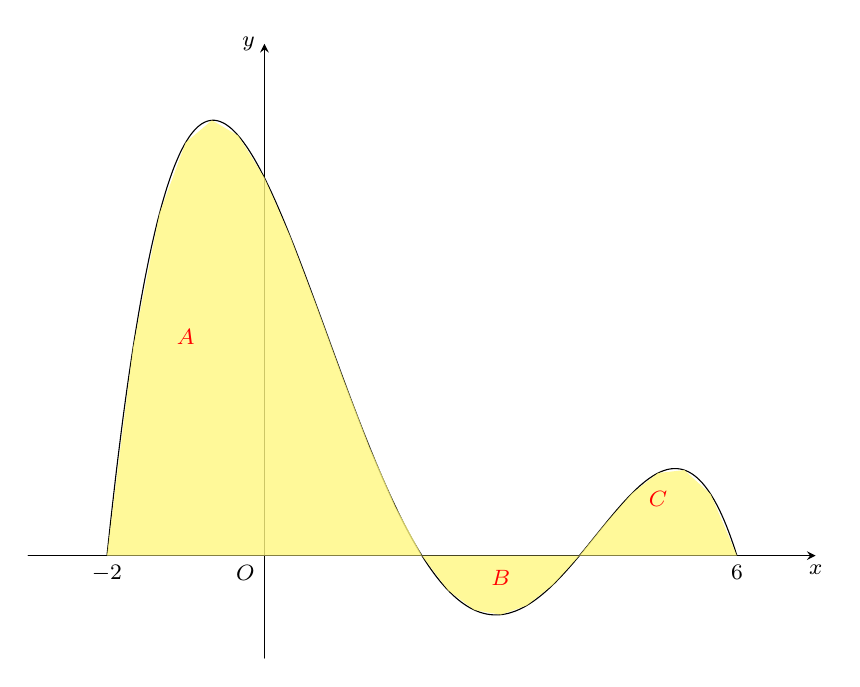
\begin{tikzpicture}[scale=1,>=stealth, font=\footnotesize, line join=round, line cap=round]
		\def\a{1} \def\b{-6} \def\c{9} \def\d{1} % Hệ số
		\def\xmin{-3} \def\xmax{7}
		\def\ymin{-1.3} \def\ymax{6.5} 
		%\draw[color=gray!50,dashed] (\xmin,\ymin) grid (\xmax,\ymax); 
		\draw[->] (\xmin,0)--(\xmax,0) node [below]{$x$};
		\draw[->] (0,\ymin)--(0,\ymax) node [left]{$y$};
		\node at (0,0) [below left]{$O$};
		\node at (-2,0) [below]{$-2$};
		\node at (6,0) [below]{$6$};
		
		\clip (\xmin+0.1,\ymin+0.1) rectangle (\xmax-0.5,\ymax-0.1);
		\draw[smooth,samples=300][domain=-2:6] plot(\x,{0-1/20*((\x)+2)*((\x)-6)*((\x)-2)*((\x)-4)});
		\fill[color=yellow!50,opacity=0.8] plot[domain=-2:6](\x,{0-1/20*((\x)+2)*((\x)-6)*((\x)-2)*((\x)-4)})--cycle;
		\node at (-1,3) [below][color=red]{$A$};
		\node at (3,-0.5) [above][color=red]{$B$};
		\node at (5,0.5) [above][color=red]{$C$};
\end{tikzpicture}}
\loigiai{
	Ta có $\displaystyle\int\limits_{-2}^2{\left[ f(2x+2)+1 \right]\mathrm{\,d}x}=\displaystyle\int\limits_{-2}^2{f(2x+2)\mathrm{\,d}x}+4$.\\
	Xét $I_1=\displaystyle\int\limits_{-2}^2{f(2x+2)\mathrm{\,d}x}$.\\
	Đặt $t=2x+2\Rightarrow \mathrm{\,d}t=2\mathrm{\,d}x\Rightarrow \mathrm{\,d}x=\dfrac{\mathrm{\,d}x}{2}$.\\ Đổi cận $x=-2\Rightarrow t=-2$; $x=2\Rightarrow t=6$.\\
	Suy ra $I_1=\dfrac{1}{2}\displaystyle\int\limits_{-2}^6{f(t)\mathrm{\,d}t}$.\\
	$\Rightarrow {I_1}=\dfrac{1}{2}\left( \displaystyle\int\limits_{-2}^{x_1}{f(t)\mathrm{\,d}t}+\int\limits_{x_1}^{x_2}{f(t)\mathrm{\,d}t}+\displaystyle\int\limits_{x_2}^6{f(t)\mathrm{\,d}t} \right)=\dfrac{1}{2}\left( {S_A}-S_B+S_C \right)=\dfrac{1}{2}\left( 32-2+3 \right)=\dfrac{33}{2}$, với $x_1$, $x_2$ là các hoành độ giao điểm của đồ thị hàm số $y=f(x)$ với trục hoành $(-2<x_1<x_2<6)$.\\
	Vậy $\displaystyle\int\limits_{-2}^2{\left[ f(2x+2)+1 \right]\mathrm{\,d}x=}{I_1}+4=\dfrac{33}{2}+4=\dfrac{41}{2}$.\\
}
\end{ex}

\begin{ex}%[Võ Thị Thùy Trang]%[2D3G3-1] cau 12
	\immini{
		Cho hàm số $f\left( x \right)$. Đồ thị của hàm số $y=f'\left( x \right)$ trên $\left[ -3;3 \right]$ như hình vẽ (phần đường cong của đồ thị là một phần của parabol $y=a{x^2}+bx+c$).\\
		Biết $f\left( 3 \right)=0$, giá trị của $f\left( -1 \right)+f\left( 1 \right)$ bằng
		\choice
		{\True  $-\dfrac{16}{3}$}
		{ $-\dfrac{8}{3}$}
		{ $\dfrac{16}{3}$}
		{ $\dfrac{8}{3}$}
	}
{\begin{tikzpicture}[scale=1,>=stealth, font=\footnotesize, line join=round, line cap=round]
		\def\a{-1} \def\b{4} \def\c{-3} % Hệ số
		\def\xmin{-3.5} \def\xmax{4}
		\def\ymin{-2} \def\ymax{2.5}
		%\draw[color=gray!50,dashed] (\xmin,\ymin) grid (\xmax,\ymax);
		\draw[->] (\xmin,0)--(\xmax,0) node [below]{$x$};
		\draw[->] (0,\ymin)--(0,\ymax) node [left]{$y$};
		\node at (0,0) [below left]{$O$};
		\clip (\xmin+0.1,\ymin+0.1) rectangle (\xmax-0.5,\ymax-0.1);
		\draw[smooth,samples=300][domain=1:3.5] plot(\x,{\a*(\x)^2+\b*(\x)+\c});
		\draw (-3,0)--(0,2)--(1,0);
		\draw[dashed] (2,0)--(2,1)--(0,1);
		\foreach \x in {-3,1,2,3}
		\draw[thin] (\x,1pt)--(\x,-1pt) node [below] {$\x$};
		\foreach \y in {1,2}
		\draw[thin] (1pt,\y)--(-1pt,\y) node [left] {$\y$};
\end{tikzpicture}}	
\loigiai{
	Ta có đường cong Parabol có đỉnh $\left(2;1\right)$ và đi qua hai điểm $\left(1;0\right),\left(3;0\right)$ nên có phương trình\\
	$y=f'\left( x \right)=-x^2+4x-3$.\\
	Suy ra $\displaystyle\int\limits_1^3{f'\left( x \right)\mathrm{\,d}x}=\displaystyle\int\limits_1^3{\left( -x^2+4x-3 \right)\mathrm{\,d}x}=\dfrac{4}{3}\Leftrightarrow f\left( 3 \right)-f\left( 1 \right)=\dfrac{4}{3}\Rightarrow f\left( 1 \right)=-\dfrac{4}{3}$.\\
	Đường thẳng $d$ đi qua hai điểm $\left(-3;0 \right),~\left(0;2 \right)$ nên có phương trình $y=\dfrac{2}{3}x+2$.\\
	Suy ra với điểm có hoành độ $x=-1$ thuộc $d\Rightarrow $ tung độ $y=\dfrac{4}{3}$.\\
	Suy ra $\displaystyle\int\limits_{-1}^1{f'\left( x \right)\mathrm{\,d}x}=f\left( 1 \right)-f\left( -1 \right)=\left( \dfrac{4}{3}+2 \right).\dfrac{1}{2}+\dfrac{1}{2}\cdot 2\cdot 1=\dfrac{8}{3}\Rightarrow f\left( -1 \right)=f\left( 1 \right)-\dfrac{8}{3}=-4$.\\
	Vậy $f\left( -1 \right)+f\left( 1 \right)=-4-\dfrac{4}{3}=-\dfrac{16}{3}$.}	
\end{ex}
\begin{ex}%[Võ Thị Thùy Trang]%[2D3G3-1] cau 13
	\immini{
		Cho hàm số $y=f\left( x \right)$ liên tục trên $\mathbb{R}$ và có đồ thị như hình vẽ. Biết rằng diện tích các hình phẳng $\left( A \right)$ và $\left( B \right)$ lần lượt bằng $15$ và $3$. Tích phân $\displaystyle\int\limits_{\frac{1}{e}}^1{\dfrac{1}{x}f\left( 3\ln x+2 \right)\mathrm{\,d}x}$ bằng
		\choice
		{\True  $4$}
		{ $-4$}
		{ $6$}
		{ $-6$}
	}
		{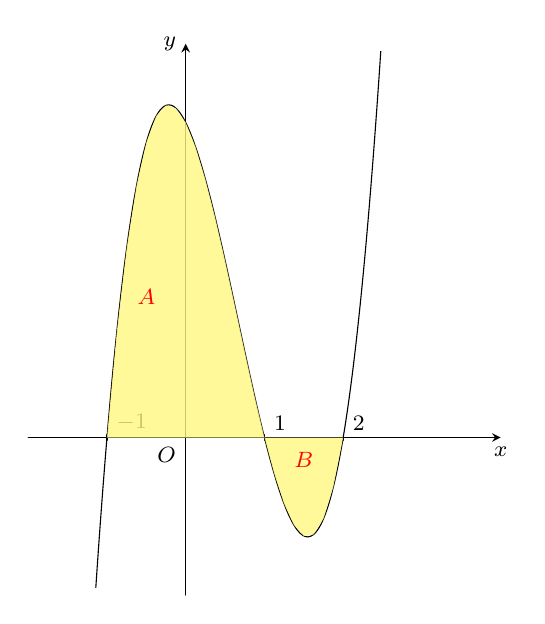
\begin{tikzpicture}[scale=1,>=stealth, font=\footnotesize, line join=round, line cap=round]
				\def\a{1} \def\b{-6} \def\c{9} \def\d{1} % Hệ số
				\def\xmin{-2} \def\xmax{4}
				\def\ymin{-2} \def\ymax{5} 
				%\draw[color=gray!50,dashed] (\xmin,\ymin) grid (\xmax,\ymax); 
				\draw[->] (\xmin,0)--(\xmax,0) node [below]{$x$};
				\draw[->] (0,\ymin)--(0,\ymax) node [left]{$y$};
				\node at (0,0) [below left]{$O$};
				\clip (\xmin+0.1,\ymin+0.1) rectangle (\xmax-0.5,\ymax-0.1);
				\draw[smooth,samples=300] plot(\x,{2*((\x)^(2.0)-1)*((\x)-2)});
				\foreach \x in {-1,1,2}
				\draw[thin] (\x,1pt)--(\x,-1pt) node [above right] {$\x$};
				\fill[color=yellow!50,opacity=0.8] plot[domain=-1:2](\x,{2*((\x)^(2.0)-1)*((\x)-2)})--cycle;
				\node at (-.5,2) [below][color=red]{$A$};
				\node at (1.5,-0.5) [above][color=red]{$B$};
		\end{tikzpicture}}
	\loigiai{
		Hình phẳng $\left( A \right)$ giới hạn bởi các đường $y=f\left( x \right)$, $y=0$, $x=-1$, $x=1$ và có phần đồ thị nằm phía trên trục hoành nên ta có $\displaystyle\int\limits_{-1}^1{f\left( x \right)\mathrm{\,d}x}=15$.\\
		Hình phẳng $\left( B \right)$ giới hạn bởi các đường $y=f\left( x \right)$, $y=0$, $x=1$, $x=2$ và có phần đồ thị nằm phía dưới trục hoành nên ta có $\displaystyle\int\limits_1^2{f\left( x \right)\mathrm{\,d}x}=-3$.\\
		Xét tích phân $I=\displaystyle\int\limits_{\frac{1}{e}}^1{\dfrac{1}{x}f\left( 3\ln x+2 \right)\mathrm{\,d}x}$.\\
		Đặt $t=3\ln x+2\Rightarrow \mathrm{\,d}t=\dfrac{3}{x}\mathrm{\,d}x\Rightarrow \dfrac{\mathrm{\,d}t}{3}=\dfrac{\mathrm{\,d}x}{x}$.\\
		Đổi cận\\
		Với $x=\dfrac{1}{e}\Rightarrow t=-1$.\\
		Với $x=1\Rightarrow t=2$.\\
		Do đó $I=\displaystyle\int\limits_{-1}^2{f\left( t \right)\dfrac{\mathrm{\,d}t}{3}}=\dfrac{1}{3}\displaystyle\int\limits_{-1}^2{f\left( t \right)\mathrm{\,d}t}=\dfrac{1}{3}\left( \displaystyle\int\limits_{-1}^1{f\left( t \right)\mathrm{\,d}t}+\displaystyle\int\limits_1^2{f\left( t \right)\mathrm{\,d}t} \right)=\dfrac{1}{3}\left( 15-3 \right)=4$.}
\end{ex}
\begin{ex}%[Võ Thị Thùy Trang]%[2D3G3-1] cau 14
	\immini{
			Cho hàm số bậc ba $f\left( x \right)=a{x^3}+bx^2+bx+2$ và parabol $g\left( x \right)=mx^2+nx+p$ có đồ thị như hình vẽ bên.
		Biết hai đồ thị tiếp xúc nhau tại điểm có hoành độ bằng $-1$. Diện tích phần hình phẳng phần được gạch chéo nằm trong khoảng
		\choice
		{ $\left(1{,}588;1{,}592\right)$}
		{ $\left(1{,}551;1{,}574\right)$}
		{\True  $\left(1{,}542;1{,}551\right)$}
		{ $\left(1{,}574;1{,}588\right)$}
	}
	{	\begin{tikzpicture}[scale=1,>=stealth, font=\footnotesize, line join=round, line cap=round]
			\def\a{1} \def\b{-5/3} \def\c{-5/3} \def\d{2} % Hệ số
			\def\e{-31/12} \def\f{-1/2} \def\g{37/12} \def\d{2} % Hệ số
			\def\xmin{-2} \def\xmax{4}
			\def\ymin{-1.5} \def\ymax{4} 
			%		\draw[color=gray!50,dashed] (\xmin,\ymin) grid (\xmax,\ymax); 
			\draw[->] (\xmin,0)--(\xmax,0) node [below]{$x$};
			\draw[->] (0,\ymin)--(0,\ymax) node [left]{$y$};
			\node at (0,0) [below left]{$O$};
			\node at (1,0) [above right]{$1$};
			\node at (2,0) [below right]{$2$};
			\node at (3.5,4) [below left]{$f(x)$};
			\node at (0,3) [above right]{$g(x)$};
			\draw[dashed](-1,0)node[below]{$-1$}--(-1,1)--(0,1)node[right]{$1$};
			\clip (\xmin+0.1,\ymin+0.1) rectangle (\xmax-0.5,\ymax-0.1);
			\draw[smooth,samples=300] plot(\x,{\a*(\x)^3+\b*(\x)^2+\c*(\x)+\d});
			\draw[smooth,samples=300] plot(\x,{\e*(\x)^2+\f*(\x)+\g});
			\fill[pattern=north east lines,opacity=0.8] plot[domain=-1:1](\x,{\a*(\x)^3+\b*(\x)^2+\c*(\x)+\d})--(1,0)--plot[domain=1:-1](\x,{\e*(\x)^2+\f*(\x)+\g})(-1.,1.) -- cycle;
	\end{tikzpicture}}
	\loigiai{
		Cho đồ thị hàm số bậc ba đi qua hai điểm $\left( -1\,;\,1 \right)$, $\left( 2\,;\,0 \right)$ có $\left\{ \begin{aligned}
			& -a+2=1 \\
			& 8a+4b+2b+2=0 \\
		\end{aligned} \right.\Leftrightarrow \left\{ \begin{aligned}
			& a=1 \\
			& b=-\dfrac{5}{3}. \\
		\end{aligned} \right.$\\
		Suy ra $f\left( x \right)=x^3-\dfrac{5}{3}{x^2}-\dfrac{5}{3}x+2$.\\
		Cho parabol đi qua hai điểm $\left( -1\,;\,1 \right)$, $\left( 1\,;\,0 \right)$ ta có $\left\{ \begin{aligned}
			& m-n+p=1 \\
			& m+n+p=0 \\
		\end{aligned} \right.\Leftrightarrow \left\{ \begin{aligned}
			& n=-\dfrac{1}{2} \\
			& m+p=\dfrac{1}{2}. \\
		\end{aligned} \right.$\\
		Lại có $f'\left( -1 \right)={g}'\left( -1 \right)\Leftrightarrow \left[ 3{{\left( -1 \right)}^2}-\dfrac{10}{3}\left( -1 \right)-\dfrac{5}{3} \right]=\left[ 2m\left( -1 \right)+n \right]\Leftrightarrow \dfrac{14}{3}=-2m+n$.\\
		Từ đó suy ra $m=-\dfrac{31}{12}$, $n=-\dfrac{1}{2}$, $p=\dfrac{37}{12}\Rightarrow g\left( x \right)=-\dfrac{31}{12}{x^2}-\dfrac{1}{2}x+\dfrac{37}{12}$.\\
		Ta dễ dàng tìm được giao điểm thứ hai của hai đồ thị là nghiệm của phương trình\\
		$x^3-\dfrac{5}{3}{x^2}-\dfrac{5}{3}x+2=-\dfrac{31}{12}{x^2}-\dfrac{1}{2}x+\dfrac{37}{12}\Leftrightarrow \hoac{& x=-1 \\
			& x=\dfrac{13}{12}.}$\\
		Suy ra diện tích hình phẳng cần tính là $$\displaystyle\int\limits_{-1}^{\tfrac{13}{12}}{\left| \left( {x^3}-\dfrac{5}{3}{x^2}-\dfrac{5}{3}x+2 \right)-\left( -\dfrac{31}{12}{x^2}-\dfrac{1}{2}x+\dfrac{37}{12} \right) \right|}\mathrm{\,d}x\approx 1,57.$$}
\end{ex}
\begin{ex}%[Võ Thị Thùy Trang]%[2D3G2-4] cau 15
	Cho hàm số $f\left( x \right)$ có đạo hàm $f'\left( x \right)=\left( x-1 \right)\left( {x^2}-3 \right)\left( {x^4}-1 \right)$ với mọi $x\in \mathbb{R}$. So sánh $f\left( -2 \right)$; $f\left( 0 \right)$; $f\left( 2 \right)$ ta được
	\choice
	{\True  $f\left( 2 \right)<f\left( 0 \right)<f\left( -2 \right)$}
	{ $f\left( 0 \right)<f\left( -2 \right)<f\left( 2 \right)$.
	}
	{ $f\left( -2 \right)<f\left( 2 \right)<f\left( 0 \right)$}
	{ $f\left( -2 \right)<f\left( 0 \right)<f\left( 2 \right)$}
	\loigiai{
		Ta có $f'\left( x \right)=\left( x-1 \right)\left( {x^2}-3 \right)\left( {x^4}-1 \right)$=$x^7-x^6-3x^5+3x^4-x^3+x^2+3x-3$.
		\begin{itemize}
			\item $I_1=\displaystyle\int\limits_{-2}^0{f'\left( x \right)\mathrm{\,d}x}=\displaystyle\int\limits_{-2}^0{\left( {x^7}-x^6-3x^5+3x^4-x^3+x^2+3x-3 \right)\mathrm{\,d}x}=\dfrac{-464}{105}<0$\\
			$\Rightarrow f\left( 0 \right)-f\left( -2 \right)<0\Rightarrow f\left( 0 \right)<f\left( -2 \right)$.
			\item $I_2=\displaystyle\int\limits_0^2{f'\left( x \right)\mathrm{\,d}x}=\displaystyle\int\limits_0^2{\left( {x^7}-x^6-3x^5+3x^4-x^3+x^2+3x-3 \right)\mathrm{\,d}x}=\dfrac{-44}{105}<0$ $\Rightarrow f\left( 2 \right)-f\left( 0 \right)<0\\ \Rightarrow f\left( 2 \right)<f\left( 0 \right)$.
		\end{itemize}
		Vậy $f\left( 2 \right)<f\left( 0 \right)<f\left( -2 \right)$.}
\end{ex}
\begin{ex}%[Võ Thị Thùy Trang]%[2D3G3-1] cau 16
	\immini{
		Cho hàm số $y=f\left( x \right)$ có đồ thị như hình vẽ dưới đây (phần cong của đồ thị là một phần của parabol $y=a{x^2}+bx+c$). Tính diện tích hình phẳng giới hạn bởi đồ thị $y=f\left( x \right)$, $y=0$, $x=-2$, $x=3$.
	\choice
	{ $S=\dfrac{43}{2}$}
	{ $S=\dfrac{95}{6}$}
	{\True  $S=\dfrac{97}{6}$}
	{ $S=\dfrac{53}{3}$}
}
{\begin{tikzpicture}[scale=.5,>=stealth, font=\footnotesize, line join=round, line cap=round]
		%	\draw[color=gray!50,dashed] (-5,-5) grid (5,5);
		\draw[->] (-5,0)--(5,0) node [below]{$x$};
		\draw[->] (0,-1)--(0,5) node [left]{$y$};
		\node at (0,0) [above left]{$O$};
		\clip (-5,-5) rectangle (6,6);
		\draw (-3,0)--(0,4)--(1,3);
		%	\draw[smooth,samples=300][domain=-0.3:3.3] plot(\x,{{-1}*\x+4});
		\draw[smooth,samples=300][domain=1:4.13] plot(\x,{-(\x-2)^2+4});
		\draw[dashed]  (1,0)--(1,3)--(0,3) (2,0)--(2,4)--(0,4) ;
		\draw (-2,0)--(-2,1.33)  (3,0)--(3,3);
		\foreach \x in {-3,-2,1,2,3,4}
		\draw[thin] (\x,1pt)--(\x,-1pt) node [below] {$\x$};
		\foreach \y in {1,2,3,4}
		\draw[thin] (1pt,\y)--(-1pt,\y) node [left] {$\y$};		
\end{tikzpicture}}
	\loigiai{
		Dựa vào đồ thị ta có diện tích hình phẳng giới hạn bởi ${{\Delta }_1}$, ${{\Delta }_2}$, parabol $\left( P \right)$, $x=-2$, $x=3$.\\
		Với ${{\Delta }_1}$qua $E\left( -3;\,0 \right)$, $D\left( 0;4 \right)$nên có pt $y=\dfrac{4}{3}x+4$; ${{\Delta }_2}$ qua $D\left( 0;4 \right)$, $C\left( 1;\,3 \right)$ nên có phương trình $y=-x+4$; $\left( P \right)\colon y=a{x^2}+bx+c$ qua $C\left( 1;\,3 \right)$ và có đỉnh $A\left( 2;4 \right)$ nên\\ $\left\{ \begin{aligned}
			& a+b+c=3 \\
			& \dfrac{-b}{2a}=2 \\
			& 4a+2b+c=4 \\
		\end{aligned} \right.\Leftrightarrow \left\{ \begin{aligned}
			& a=-1 \\
			& b=4 \\
			& c=0 \\
		\end{aligned} \right.\Rightarrow y=-x^2+4x$.\\
		Vậy $S=\displaystyle\int\limits_{-2}^3{\left| f\left( x \right) \right| \mathrm{\,d}x}=\displaystyle\int\limits_{-2}^3{f\left( x \right) \mathrm{\,d}x}=\displaystyle\int\limits_{-2}^0{\left( \dfrac{4}{3}x+4 \right) \mathrm{\,d}x+\displaystyle\int\limits_0^1{\left( -x+4 \right) \mathrm{\,d}x+\int\limits_1^3{\left( -x^2+4x \right) \mathrm{\,d}x}}=\dfrac{97}{6}}$.}
\end{ex}
\begin{ex}%[Võ Thị Thùy Trang]%[2D3G3-1] cau 17
\immini{
	Cho hình cong $\left( H \right)$ giới hạn bởi các đường $y=\dfrac{2}{x}$, $x=1$, $x=4$ và trục hoành. Đường thẳng $x=k\left( 1<k<4 \right)$ chia $\left( H \right)$ thành hai phần có diện tích là $S_1$ và $S_2$ như
	hình vẽ bên, biết $S_1=3S_2$. Giá trị của $k$ là?
	
	\choice
	{\True  $\sqrt{8}$}
	{ $\sqrt{6}$}
	{ $\sqrt{7}$}
	{ $\sqrt{5}$}
}
{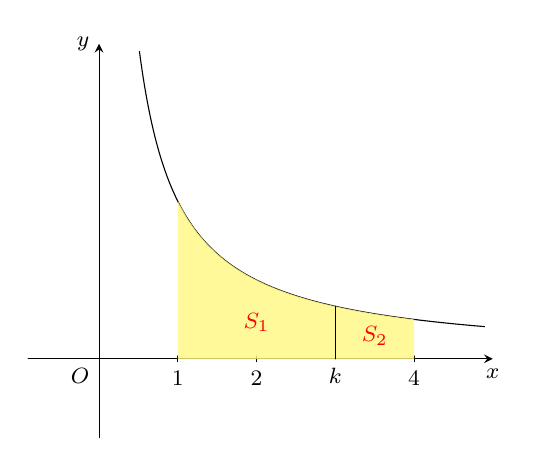
\begin{tikzpicture}[scale=1,>=stealth, font=\footnotesize, line join=round, line cap=round]
		\def\xmax{5} \def\ymin{-1} \def\ymax{4}
		%	\draw[color=gray!50,dashed] (-0.9,\ymin) grid (\xmax,\ymax);
		\draw[->] (-0.9,0)--(\xmax,0) node [below]{$x$};
		\draw[->] (0,\ymin)--(0,\ymax) node [left]{$y$};
		\node at (0,0) [below left]{$O$};
		\clip (-0.9,\ymin) rectangle (\xmax-0.1,\ymax-0.1);
		\draw[smooth,samples=300,domain=0.03:\xmax] plot(\x,{2/(\x)});
		\foreach \x in {1,2,4}
		\draw[thin] (\x,1pt)--(\x,-1pt) node [below] {$\x$};
		\fill[color=yellow!50,opacity=0.8](4,0)-- plot[domain=4:1](\x,{2/(\x)})--(1,0)--cycle;
		\draw (3,0)node [below]{$k$}--(3,2/3);
		\node at (2,.7) [below][color=red]{$S_1$};
		\node at (3.5,0.05) [above][color=red]{$S_2$};
\end{tikzpicture}}
\loigiai{
	Ta có
	$\left\{ \begin{aligned}
		& {S_1}+S_2=\displaystyle\int\limits_1^4{\dfrac{2}{x}\mathrm{\,d}x=\left. 2\ln x \right|_1^4=4\ln 2} \\
		& {S_1}=3S_2 \\
	\end{aligned} \right.\Leftrightarrow \left\{ \begin{aligned}
		& {S_1}=3\ln 2 \\
		& {S_2}=\ln 2.\\
	\end{aligned} \right.$\\
	Ta có $\ln 2=S_2\Leftrightarrow \ln 2=\displaystyle\int\limits_k^4{\dfrac{2}{x}\mathrm{\,d}x\Leftrightarrow \ln 2= 2\ln x\bigg|_k^4\Leftrightarrow \ln 2=4\ln 2}-2\ln k$.\\
	$\Leftrightarrow 2\ln k=3\ln 2\Leftrightarrow {k^2}=8\Leftrightarrow k=\sqrt{8}$ ($1<k<4$).\\
	Vậy $k=\sqrt{8}$.}	
\end{ex}
\begin{ex}%[Võ Thị Thùy Trang]%[2D3G3-1] cau 18
	\immini{
		Bạn An cần mua một chiếc gương có đường viền là đường Parabol bậc 2 (xem hình vẽ). Biết rằng khoảng cách đoạn $AB=60\,\text{cm}$, $OH=30\,\text{cm}$. Diện tích của chiếc gương bạn An mua là
\choice
{ $900\left( \text{c}{{\text{m}}^2} \right)$}
{ $1000\left( \text{c}{{\text{m}}^2} \right)$}
{ $1400\left( \text{c}{{\text{m}}^2} \right)$}
{\True  $1200\left( \text{c}{{\text{m}}^2} \right)$}
}
{\begin{tikzpicture}[scale=1,>=stealth, font=\footnotesize, line join=round, line cap=round]
		\def\a{-1} \def\b{0} \def\c{+4} % Hệ số
		\def\xmin{-2.2} \def\xmax{2.5}
		\def\ymin{-0.3} \def\ymax{4.2}
		%	\draw[color=gray!50,dashed] (\xmin,\ymin) grid (\xmax,\ymax);
		\node at (-2,0) [below][color=red]{$A$};
		\node at (2,0) [below][color=red]{$B$};
		\draw[->] (\xmin,0)--(\xmax,0) node [below]{$x$};
		\draw[->] (0,\ymin)--(0,\ymax) node [left]{$H$};
		\node at (0,0) [below left]{$O$};
		\clip (\xmin+0.1,\ymin+0.1) rectangle (\xmax-0.5,\ymax-0.1);
		\draw[smooth,samples=300][domain=-2.5:2.5] plot(\x,{\a*(\x)^2+\b*(\x)+\c});
\end{tikzpicture}}
\loigiai{\immini{
		\begin{itemize}
			\item  Gắn hệ trục tọa độ $Oxy$ như hình vẽ.
			\item  Ta có $O\left( 0;0 \right)$; $A\left( -30;0 \right)$; $B\left( 30;0 \right)$;$H\left( 0;30 \right)$.
			\item  Phương trình Parabol có dạng $y=a{x^2}+bx+c\,\left( a\ne 0 \right)$.
			\item  Parabol đi qua các điểm $A,\,B,\,H$ nên ta có hệ phương trình \\
			$\left\{ \begin{aligned}
				& {{\left( -30 \right)}^2}a-30b+c=0 \\
				& {{30}^2}a+30b+c=0 \\
				& c=30 \\
			\end{aligned} \right.\Leftrightarrow \left\{ \begin{aligned}
				& a=-\dfrac{1}{30} \\
				& b=0 \\
				& c=30. \\
			\end{aligned} \right.\\
		\Rightarrow $Phương trình Parabol là $y=-\dfrac{1}{30}{x^2}+30$.\\
		\end{itemize}
			
	}
{\begin{tikzpicture}[scale=1,>=stealth, font=\footnotesize, line join=round, line cap=round]
		\def\a{-1} \def\b{0} \def\c{+4} % Hệ số
		\def\xmin{-2.2} \def\xmax{2.5}
		\def\ymin{-0.3} \def\ymax{4.2}
		%	\draw[color=gray!50,dashed] (\xmin,\ymin) grid (\xmax,\ymax);
		\node at (-2,0) [below][color=red]{$A$};
		\node at (2,0) [below][color=red]{$B$};
		\draw[->] (\xmin,0)--(\xmax,0) node [below]{$x$};
		\draw[->] (0,\ymin)--(0,\ymax) node [left]{$H$};
		\node at (0,0) [below left]{$O$};
		\clip (\xmin+0.1,\ymin+0.1) rectangle (\xmax-0.5,\ymax-0.1);
		\draw[smooth,samples=300][domain=-2.5:2.5] plot(\x,{\a*(\x)^2+\b*(\x)+\c});
\end{tikzpicture}}
	Vậy diện tích chiếc gương là $S=\displaystyle\int\limits_{-30}^{30}{\left( -\dfrac{1}{30}{x^2}+30 \right)\mathrm{\,d}x}$ $=1200\,\left( \text{c}{{\text{m}}^{\text{2}}} \right)$.\\
	Trắc nghiệm nhanh: Diện tích Parabol có đáy $R=\dfrac{AB}{2}=30$ và đường cao $h=OH=30$ là $S=\dfrac{4}{3}Rh$ $=\dfrac{4}{3}\cdot 30\cdot 30=1200\,\left( \text{c}{{\text{m}}^{\text{2}}} \right)$.}	
\end{ex}
\begin{ex}%[Võ Thị Thùy Trang]%[2D3G3-1] cau 19
	\immini{
			Cho đường thẳng $y=2x$ và parabol $y=x^2+c$ ($c$ là tham số thực dương). Gọi $S_1$ và $S_2$ lần lượt là diện tích của hai hình phẳng được gạch chéo trong hình vẽ. Khi $S_1=S_2$ thì $c$ gần với số nào nhất sau đây?
		\choice
		{ $2$}
		{ $0$}
		{\True  $1$}
		{ $3$}
	}
{\begin{tikzpicture}[scale=.65,>=stealth, font=\footnotesize, line join=round, line cap=round]
		%	\draw[color=gray!50,dashed] (-5,-5) grid (5,5);
		\draw[->] (-2,0)--(4,0) node [below]{$x$};
		\draw[->] (0,-1)--(0,6) node [left]{$y$};
		\node at (0,0) [above left]{$O$};
		\clip (-5,-5) rectangle (6,6);
		\draw[smooth,samples=300][domain=-0.3:3.3] plot(\x,{2*\x});
		\draw[smooth,samples=300][domain=-0.3:3.3] plot(\x,{(\x-0.5)^2+1});
		\fill[color=green!50,opacity=0.8] {[smooth,samples=50,domain=0.0:2.5] plot(\x,{2*(\x)})} -- (2.5,5.) {[smooth,samples=50,domain=2.5:0.0] -- plot(\x,{((\x)-0.5)^(2)+1})} -- (0.,0.) -- cycle;
		\node at (3.15,5) [below][color=red]{$y=2x$};
		\node at (2.85,2.5) [above][color=red]{$y=x^2+c$};
		\draw[->] (0.2,2)node [above][color=red]{$S_1$}--(0.2,0.65);
		\draw[->] (1.3,4.2)node [above][color=red]{$S_2$}--(1.3,2.25);
\end{tikzpicture}}
\loigiai{\immini{
			Phương trình hoành độ giao điểm của đường thẳng và parabol\\
		$x^2+c=2x\Leftrightarrow {x^2}-2x+c=0$.\\
		Để phương trình có hai nghiệm phân biệt thì $\Delta '=1-c>0\Leftrightarrow c<1$.\\
		Theo Vi-et ta có $\left\{ \begin{aligned}
			& {x_1}+x_2=2 \\
			& {x_1}\cdot x_2=c \\
		\end{aligned} \right.\Leftrightarrow \left\{ \begin{aligned}
			& {x_1}=2-x_2 &\quad(1) \\
			& {x_1}.x_2=c. &\quad( 2) \\
		\end{aligned} \right.$	}
	{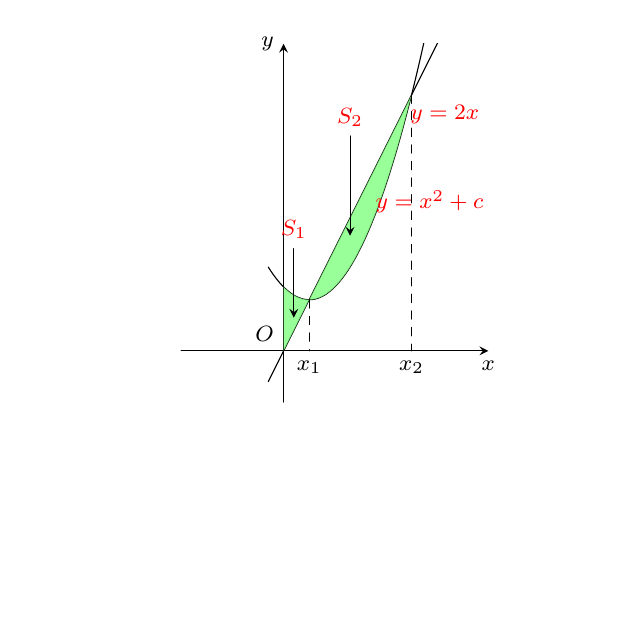
\begin{tikzpicture}[scale=.65,>=stealth, font=\footnotesize, line join=round, line cap=round]
			%	\draw[color=gray!50,dashed] (-5,-5) grid (5,5);
			\draw[->] (-2,0)--(4,0) node [below]{$x$};
			\draw[->] (0,-1)--(0,6) node [left]{$y$};
			\node at (0,0) [above left]{$O$};
			\clip (-5,-5) rectangle (6,6);
			\draw[smooth,samples=300][domain=-0.3:3.3] plot(\x,{2*\x});
			\draw[smooth,samples=300][domain=-0.3:3.3] plot(\x,{(\x-0.5)^2+1});
			\fill[color=green!50,opacity=0.8] {[smooth,samples=50,domain=0.0:2.5] plot(\x,{2*(\x)})} -- (2.5,5.) {[smooth,samples=50,domain=2.5:0.0] -- plot(\x,{((\x)-0.5)^(2)+1})} -- (0.,0.) -- cycle;
			\node at (3.15,5) [below][color=red]{$y=2x$};
			\node at (2.85,2.5) [above][color=red]{$y=x^2+c$};
			\draw[->] (0.2,2)node [above][color=red]{$S_1$}--(0.2,0.65);
			\draw[->] (1.3,4.2)node [above][color=red]{$S_2$}--(1.3,2.25);
			\draw[dashed](0.5,1)--(0.5,0)node [below]{$x_1$};
			\draw[dashed](2.5,5)--(2.5,0)node [below]{$x_2$};
	\end{tikzpicture}}
	Do $S_1=S_2\Leftrightarrow \displaystyle\int\limits_0^{x_1}{\left( {x^2}+c-2x \right)\mathrm{\,d}x}=-\displaystyle\int\limits_{x_1}^{x_2}{\left( {x^2}+c-2x \right)\mathrm{\,d}x}$\\
$\begin{aligned}
	& \Leftrightarrow \displaystyle\int\limits_0^{x_1}{\left( {x^2}-2x+c \right)\mathrm{\,d}x}+\displaystyle\int\limits_{x_1}^{x_2}{\left( {x^2}-2x+c \right)\mathrm{\,d}x}=0\Leftrightarrow \displaystyle\int\limits_0^{x_2}{\left( {x^2}-2x+c \right)\mathrm{\,d}x}=0 \\
	& \Leftrightarrow \left( \dfrac{x^3}{3}-x^2+cx \right)\left| \begin{aligned}
		& {x_2} \\
		& 0 \\
	\end{aligned} \right.=0\Leftrightarrow \dfrac{x_2^3}{3}-x_2^2+c{x_2}=0\Leftrightarrow \dfrac{x_2^2}{3}-x_2+c=0\Leftrightarrow c=-\dfrac{x_2^2}{3}+x_2.\quad( 3 ) \\
\end{aligned}$\\
Thay $\left( 1 \right)$ và $\left(3\right)$ vào $\left( 2 \right)$ ta được\\
$\left( 2-x_2 \right)\cdot x_2=-\dfrac{x_2^2}{3}+x_2\Leftrightarrow 2x_2-x_2^2=-\dfrac{x_2^2}{3}+x_2\Leftrightarrow \dfrac{2}{3}x_2^2-x_2=0\Leftrightarrow \dfrac{2}{3}{x_2}-1=0\Leftrightarrow {x_2}=\dfrac{3}{2}$.\\
Thay $x_2=\dfrac{3}{2}$ vào $\left( 3 \right)\Rightarrow c=\dfrac{3}{4}=0{,}75$.
}	
\end{ex}
\begin{ex}%[Võ Thị Thùy Trang]%[2D3G3-1]cau 20
	\immini{
			Hình phẳng giới hạn bởi đồ thị hàm số $y=f\left( x \right)$ và trục hoành gồm hai phần, phần nằm phía trên trục hoành có diện tích $S_1=\dfrac{8}{3}$ và phần nằm phía dưới trục hoành có diện tích $S_2=\dfrac{5}{12}$ (tham khảo hình vẽ bên). Tính $I=\displaystyle\int\limits_{-1}^0{f\left( 3x+1 \right)}\mathrm{\,d}x$.	}
{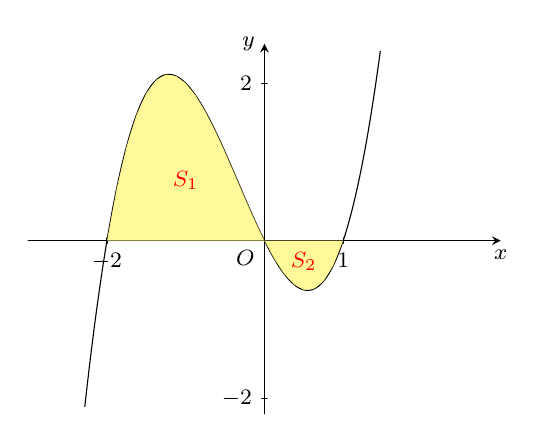
\begin{tikzpicture}[scale=1,>=stealth, font=\footnotesize, line join=round, line cap=round]
		\def\a{1} \def\b{1} \def\c{-2} \def\d{0} % Hệ số
		\def\xmin{-3} \def\xmax{3}
		\def\ymin{-2.2} \def\ymax{2.5} 
		%	\draw[color=gray!50,dashed] (\xmin,\ymin) grid (\xmax,\ymax); 
		\draw[->] (\xmin,0)--(\xmax,0) node [below]{$x$};
		\draw[->] (0,\ymin)--(0,\ymax) node [left]{$y$};
		\node at (0,0) [below left]{$O$};
		\clip (\xmin+0.1,\ymin+0.1) rectangle (\xmax-0.5,\ymax-0.1);
		\draw[smooth,samples=300] plot(\x,{\a*(\x)^3+\b*(\x)^2+\c*(\x)+\d});
		\foreach \x in {-2,1}
		\draw[thin] (\x,1pt)--(\x,-1pt) node [below] {$\x$};
		\foreach \y in {-2,2}
		\draw[thin] (1pt,\y)--(-1pt,\y) node [left] {$\y$};
		\fill[color=yellow!50,opacity=0.8] plot[domain=-2:1](\x,{\a*(\x)^3+\b*(\x)^2+\c*(\x)+\d})--cycle;
		\node at (-1,1) [below][color=red]{$S_1$};
		\node at (0.5,-0.5) [above][color=red]{$S_2$};
\end{tikzpicture}}
\choice
{ $I=\dfrac{27}{4}$}
{ $I=\dfrac{5}{3}$}
{\True  $I=\dfrac{3}{4}$}
{ $I=\dfrac{37}{36}$}
\loigiai{
	Với $I=\displaystyle\int\limits_{-1}^0{f\left( 3x+1 \right)}\mathrm{\,d}x$.\\
	Đặt $t=3x+1\Rightarrow \mathrm{\,d}t=3\mathrm{\,d}x$.\\
	Khi $\left\{ \begin{aligned}
		& x=0\Rightarrow t=1 \\
		& x=-1\Rightarrow t=-2. \\
	\end{aligned} \right.$\\
	Ta được $I=\dfrac{1}{3}\displaystyle\int\limits_{-2}^1{f\left( t \right)\mathrm{\,d}t}=\dfrac{1}{3}\displaystyle\int\limits_{-2}^1{f\left( x \right)\mathrm{\,d}x=\dfrac{1}{3}}\left(\displaystyle\int\limits_{-2}^0{f\left( x \right)dx+\displaystyle\int\limits_0^1{f\left( x \right)\mathrm{\,d}x}} \right)$.\\
	Trên đoạn $\left[ -2\,;\,0 \right]\colon f\left( x \right)\ge 0$ nên $\displaystyle\int\limits_{-2}^0{f\left( x \right)}\mathrm{\,d}x=\dfrac{8}{3}$.\\
	Trên đoạn $\left[ 0;1 \right]\colon f\left( x \right)\le 0$ nên $\int\limits_0^1{f\left( x \right)}\mathrm{\,d}x=-\dfrac{5}{12}$.\\
	Vậy $I=\dfrac{1}{3}\left(\displaystyle\int\limits_{-2}^0{f\left( x \right)\mathrm{\,d}x+\displaystyle\int\limits_0^1{f\left( x \right)\mathrm{\,d}x}} \right)=\dfrac{1}{3}\left( \dfrac{8}{3}-\dfrac{5}{12} \right)=\dfrac{3}{4}$.}	
\end{ex}
\Closesolutionfile{ans}
%======================
\subsection{Bảng đáp án}
\inputansbox{8}{ans/ANS-DANG-44}